\documentclass[headrule,footrule]{foils}

%%
%%%  Macros
%%%
\newcommand{\logo}{HG2002 (2020)}
\usepackage[hidelinks]{hyperref}

\newcommand{\header}[3]{%
  \title{\vspace*{-2ex} \large 
    HG2002 Semantics and Pragmatics
% \thanks{Creative
%       Commons Attribution License: 
%       you are free to share and adapt as long as you give 
%       appropriate credit and add no additional restrictions: 
%       \protect\url{https://creativecommons.org/licenses/by/4.0/}.
%     }
    \\[2ex] \Large  \emp{#2} \\ \emp{#3}}
  \author{\blu{Francis Bond}   \\ 
    \normalsize  \textbf{Division of Linguistics and Multilingual Studies}\\
    \normalsize  \url{http://www3.ntu.edu.sg/home/fcbond/}\\
    \normalsize  \texttt{bond@ieee.org}}
  \MyLogo{\logo}
  % \MyLogo{奈良女子大学:欧米言語情報理論II}
  \date{#1
    \\  \url{https://bond-lab.github.io/Semantics-and-Pragmatics/}
\\[.5ex] \footnotesize Creative  Commons Attribution License:  you are free to share and adapt 
\\[-.25ex] \footnotesize   as long as you give    appropriate credit and add no
additional restrictions: 
\\ \small  \protect\url{https://creativecommons.org/licenses/by/4.0/}.
}
  % \renewcommand{\logo}{#2}
  % \special{! /pdfmark where
  %   {pop} {userdict /pdfmark /cleartomark load put} ifelse
  %   [ /Author (Francis Bond)
  %   /Title (#1: #2)
  %   /Subject (HG2002: Semantics and Pragmatics)
  %   /Keywords (Semantics, Pragmatics, Meaning)
  %   /DOCINFO pdfmark}
  %   }
  \hypersetup{%
    final       = true,
    colorlinks  = true,
    urlcolor    = blue,
    citecolor   = blue,
    linkcolor   = MidnightBlue,
    unicode     = true,
    pdfauthor   = {Francis Bond},
    pdfkeywords = {Semantics, Pragmatics, Meaning},
    pdftitle    = {#1: #2},
    pdfsubject  = {HG2002 Semantics and Pragmatics; License CC BY 4.0}
  }
}


\usepackage[a4paper,landscape]{geometry}
%\usepackage[dvips]{xcolor}
\usepackage[dvipsnames,x11names]{xcolor}
\usepackage{graphicx}
\newcommand{\blu}[1]{\textcolor{blue}{#1}}
\newcommand{\grn}[1]{\textcolor{green}{#1}}
\newcommand{\hide}[1]{\textcolor{white}{#1}}
\newcommand{\emp}[1]{\textcolor{red}{#1}}
\newcommand{\txx}[1]{\textbf{\textcolor{blue}{#1}}}
\newcommand{\lex}[1]{\textbf{\mtcitestyle{#1}}}


\usepackage{amsmath,latexsym}
\usepackage{pifont}
\renewcommand{\labelitemi}{\textcolor{violet}{\ding{227}}}
\renewcommand{\labelitemii}{\textcolor{purple}{\ding{226}}}

\newcommand{\subhead}[1]{\noindent\textbf{#1}\\[5mm]}

\newcommand{\Bad}{\emp{\raisebox{0.15ex}{\ensuremath{\mathbf{\otimes}}}}}
\newcommand{\bad}{*}

\newcommand{\com}[1]{\hfill \textnormal{(\emp{#1})}}%
\newcommand{\cxm}[1]{\hfill \textnormal{(\txx{#1})}}%
\newcommand{\cmm}[1]{\hfill \textnormal{(#1)}}%

\usepackage{relsize,xspace}
\newcommand{\into}{\ensuremath{\rightarrow}\xspace}
\newcommand{\ent}{\ensuremath{\Rightarrow}\xspace}
\newcommand{\nent}{\ensuremath{\not\Rightarrow}\xspace}
\newcommand{\tot}{\ensuremath{\leftrightarrow}\xspace}
\usepackage{url}
\newcommand{\lurl}[1]{\MyLogo{\url{#1}}}

\usepackage{mygb4e}
\let\eachwordone=\itshape
\newcommand{\lx}[1]{\textbf{\textit{#1}}}
\newcommand{\ix}{\ex\it}

\newcommand{\cen}[2]{\multicolumn{#1}{c}{#2}}
%\usepackage{times}
%\usepackage{nttfoilhead}
\newcommand{\myslide}[1]{\foilhead[-25mm]{\raisebox{12mm}[0mm]{\emp{#1}}}\MyLogo{\logo}}
\newcommand{\myslider}[1]{\rotatefoilhead[-25mm]{\raisebox{12mm}[0mm]{\emp{#1}}}}
%\newcommand{\myslider}[1]{\rotatefoilhead{\raisebox{-8mm}{\emp{#1}}}}

\newcommand{\section}[1]{\myslide{}{\begin{center}\Huge \emp{#1}\end{center}}}



\usepackage[lyons,j,e,k]{mtg2e}
\renewcommand{\mtcitestyle}[1]{\textcolor{teal}{\textsl{#1}}}
%\renewcommand{\mtcitestyle}[1]{\textsl{#1}}
\newcommand{\ja}[1]{\mtcitestyle{\makexeCJKactive #1\makexeCJKinactive}}
\newcommand{\chn}{\mtciteform}
\newcommand{\zsm}{\mtciteform}
%\newcommand{\cmn}[1]{make\cjkactive\mtciteform#1\makecjkinactive}
\newcommand{\iz}[1]{\textup{\texttt{\textcolor{blue}{\textbf{#1}}}}}
\newcommand{\con}[1]{\textsc{#1}}
\newcommand{\gm}{\textsc}
\newcommand{\cmp}[1]{{[\textsc{#1}]}}
\newcommand{\sr}[1]{\ensuremath{\langle}#1\ensuremath{\rangle}}
\usepackage[normalem]{ulem}
\newcommand{\ul}{\uline}
\newcommand{\ull}{\uuline}
\newcommand{\wl}{\uwave}
\newcommand{\vs}{\ensuremath{\Leftrightarrow}~}
%%% theta role
\newcommand{\tr}[1]{\textcolor{Chartreuse4}{\textsc{#1}}}
%%% theta grid
\newcommand{\grid}[1]{\ensuremath{\langle}\tr{#1}{\ensuremath{\rangle}}}

%%%
%%% Bibliography
%%%
\usepackage{natbib}
%\usepackage{url}
\usepackage{bibentry}
%\usepackage{CJKutf8}


\usepackage{fontenc}
\usepackage{polyglossia}
\setmainlanguage{english}
\setotherlanguages{tamil}
\setmainfont[Ligatures=TeX]{TeX Gyre Pagella}
\setsansfont[Ligatures=TeX]{TeX Gyre Heros}

\usepackage{xeCJK}
\makexeCJKinactive
\newcommand{\zh}[1]{\mtcitestyle{\makexeCJKactive #1\makexeCJKinactive}}
%\newcommand{\ja}[1]{\makexeCJKactive #1\makexeCJKinactive}
\setCJKmainfont{Noto Sans CJK JP}
\setCJKsansfont{Noto Sans CJK SC}
\setCJKmonofont{Noto Sans CJK SC}

\newfontfamily\tamilfont[Script=Tamil]{Noto Sans Tamil}
\newfontfamily\tamilfontsf[Script=Tamil]{Noto Sans Tamil}
\newcommand{\tam}[1]{\texttamil{#1}}
%%% From Tim
\newcommand{\WMngram}[1][]{$n$-gram#1\xspace}
\newcommand{\infers}{$\rightarrow$\xspace}


\usepackage{rtrees,qtree}
\renewcommand{\lf}[1]{\br{#1}{}}
\usepackage{avm}
%\avmoptions{topleft,center}
\newcommand{\ft}[1]{\textsc{#1}}
\newcommand{\val}[1]{\textit{#1}}
\newcommand{\typ}[1]{\textit{#1}}
\avmfont{\sc}
\avmvalfont{\sc}
\renewcommand{\avmtreefont}{\sc}
\avmsortfont{\it}


%%% From CSLI book
\newcommand{\mc}{\multicolumn}
\newcommand{\HD}{\textbf{H}\xspace}
\newcommand{\el}{\< \>}
\makeatother
\long\def\smalltree#1{\leavevmode{\def\\{\cr\noalign{\vskip12pt}}%
\def\mc##1##2{\multispan{##1}{\hfil##2\hfil}}%
\tabskip=1em%
\hbox{\vtop{\halign{&\hfil##\hfil\cr
#1\crcr}}}}}
\makeatletter

%\usepackage{tipa}
\usepackage{multicol}


\newcommand{\task}{\marginpar{\large ~~~\textbf{?}}}
\newcommand{\sh}[1]{\href{https://www.arthur-conan-doyle.com/index.php?title=#1}{#1}}

\usepackage{tikz}
\usepackage{tikz-qtree}



\begin{document}

\header{Lecture 3}{Word Meaning}{}\maketitle

%\include{schedule}

\myslide{Overview}

\begin{itemize}\addtolength{\itemsep}{-1ex}
\item Revision: Meaning, Thought and Reality
  \begin{itemize}
  \item Reference as a Theory of Meaning
  \item Deixis
  \item Mental Representations
  \item Words, Concepts and Thinking
  \end{itemize}
\item Defining \lex{word}
\item Problems with defining word meaning
\item Lexical Relations
  \begin{itemize}
  \item Wordnet
  \end{itemize}
\item Derivational Relations
\item Lexical Universals
\item Next week: \emp{Chapter 4: Sentence Relations and Truth}
\end{itemize}

%%%
%%% this changes each year, so keep separate
%%%
%\include{schedule}
\section{Revision: \\ Meaning, Thought and Reality}


 \myslide{Referential View}

 \begin{center}
   \setlength{\unitlength}{2mm}
   \begin{picture}(80,50)(0,0) \put(5,35){\oval(25,6)}
     \put(5,35){\makebox(0,0){\bf Speaker}}

     \put(25,25){\oval(25,6)}
     \put(25,25){\makebox(0,0){\bf Expression}} 

     \put(75,25){\oval(25,6)}
     \put(75,25){\makebox(0,0){\bf Referent}} 

     \put(37.5,25){\vector(1,0){25}}
     \put(50,20){\makebox(0,0){Denote}}

     \put(17.5,35){\vector(1,-0.15){45}}
     \put(50,35){\makebox(0,0){Refer}}

     \put(5,32){\vector(1,-0.20){17}}
     \put(3,30){\makebox(0,0){Say}}

   \end{picture}
 \end{center}

 \txx{Referential view}  is focused on direct relationships between expressions (words, sentences) and things in the world (realist view).  (More in Chapter 10)



 \myslide{Representational View}
 \begin{center}
   \setlength{\unitlength}{2mm}
   \begin{picture}(80,50)(0,0) \put(5,35){\oval(25,6)}
     \put(5,35){\makebox(0,0){\bf Speaker}}

     \put(25,25){\oval(25,6)}
     \put(25,25){\makebox(0,0){\bf Expression}} 

     \put(50,40){\oval(25,6)}
     \put(50,40){\makebox(0,0){\bf Concept}} 

     \put(75,25){\oval(25,6)}
     \put(75,25){\makebox(0,0){\bf Referent}} 


     % \put(37.5,25){\vector(1,0){25}}
     % \put(50,20){\makebox(0,0){Experience}}

     \put(25,28){\vector(1,0.35){26}}
     \put(30,33){\makebox(0,0){Denote}}

     \put(17.5,35){\vector(1,0.2){20}}
     \put(30,40){\makebox(0,0){Refer}}

     \put(5,32){\vector(1,-0.20){17}}
     \put(3,30){\makebox(0,0){Say}}

     \put(50,37){\vector(1,-0.35){26}}
     \put(75,33){\makebox(0,0){Represent}}
   \end{picture}
 \end{center}
\vspace*{-10mm}
 \txx{Representational view} is focused on how relationships between
 expressions (words, sentences) and things in the world are mediated by
 the mind (cognitive linguistics).  (More in Chapters 9 and 11)

\myslide{Two types of naming}
  \begin{itemize}
  \item \txx{The description theory}: Names are like short hands for descriptions:
\begin{quote}
  William Shakespeare = ``the playwright who wrote Hamlet''  
\end{quote}
\item \txx{The causal theory}:
Names begin with some event of naming (e.g. a christening) before
becoming commonly accepted.
\begin{quote}
  William Shakespeare = ``the guy other people call William Shakespeare''  
\end{quote}
\end{itemize}

\myslide{Mental Representations}

\begin{itemize}
\item Divide meaning into
  \begin{itemize}
  \item \txx{reference}: the relation to the world
  \item \txx{sense}: the rest of the meaning
  \end{itemize}
\item Introduce \txx{concepts}
  \begin{itemize}
  \item Represented by Necessary and Sufficient Conditions
  \item  Prototypes
    \begin{itemize}
    \item Concepts are organized in groups around a \txx{prototype}
    \item These have typical members (remembered as \txx{exemplars}) 
\item prototypes have \txx{characteristic feature}s
\item Some categories (concepts) seem to be more psychologically basic than others: \txx{basic level categories}
\end{itemize}
\end{itemize}
\end{itemize}
\myslide{What is Deixis}
\begin{itemize}
\item any linguistic element whose interpretation
  necessarily makes reference to properties of the
  extra-linguistic context in which they occur is \txx{deictic}
  \begin{description}
  \item[Person] relative to the speaker and addressee
  \item[Spatial Location] demonstratives; \ldots
  \item[Temporal Location] tense; \eng{yesterday, today, tomorrow}
  \item[Social] relative to the social status: \eng{professor, you, uncle, boy}
  \end{description}
\item Discourse deixis: referring to a linguistic expression or chunk of discourse
\end{itemize}

More than 90\% of the declarative sentences people utter are indexical
in that they involve implicit references to the speaker, addressee,
time and/or place of utterance in expressions like first and second
person pronouns, demonstratives, tenses, and adverbs like here, now,
yesterday (Bar-Hillel 1954: 366).

\myslide{Spatial Deixis}
\MyLogo{Interrogative often not included}
\begin{itemize}
\item Two (three) way systems (English, \ldots)
  \\[2ex] \begin{tabular}{llll}
    \txx{proximal} &\lex{this} & \lex{here} &close to the speaker\\
    \txx{distal} &\lex{that} & \lex{there} & far to the speaker \\
    \txx{interrogative} &\lex{what} & \lex{where} & 
  \end{tabular}
\item Three (four) way systems (Japanese, \ldots)
    \\[2ex] \begin{tabular}{llll}
      \txx{proximal}& \lex{kore} ``this'' & \lex{koko} ``here'' & close to speaker\\
      \txx{medial} &\lex{sore} ``that''   & \lex{soko} ``there'' &close to addressee\\
      \txx{distal} &\lex{are} ``that'' & \lex{asoko} ``over there'' &far from both\\
      \txx{interrogative} & \lex{dore} ``which'' & \lex{doko} ``where'' &
    \end{tabular}
  \item Can decompose: \lex{this} ``this thing'', \lex{here} ``this place''
\end{itemize}


\myslide{Person Deixis}

\begin{itemize}
\item Commonly a three way division
\\[2ex]  \begin{tabular}{lll}
    First Person & Speaker & \lex{I} \\
    Second Person & Addressee & \lex{you} \\
    Third Person & Other & \lex{he/she/it} \\
  \end{tabular}
\item Often combined with
  \begin{itemize}
  \item \txx{gender}: \lex{he/she/it }
  \item \txx{number}: \lex{I/we}, 
    \lex{'anta} ``you:m'', \lex{'antumaa} ``you:dual'',  \lex{'antum} ``you:m:pl''
    \\ (Arabic)
  \item \txx{inclusion}: \lex{n\'uy} ``we including you'',  \lex{n\'{\i}i} ``we excluding you'' (Zayse)
  \item \txx{honorification}: \lex{kimi} ``you:inferior'', \lex{anata} ``you:equal'',
    \\ don't use pronouns for superiors: \lex{sensei} ``teacher'', \ldots (Japanese)
  \end{itemize}
\end{itemize}

\myslide{Social Deixis}

In European languages, a two-way choice in 2nd person pronominal
reference is known as the T/V distinction, based on the French forms
for ``you''.

\begin{itemize}
\item T/V distinctions in European languages
\\[2ex]  \begin{tabular}{lll}
    & Familiar 2sg & Polite 2sg \\ \hline
    French & tu & vous \\
    German & du & Sie \\
    Spanish & t\'u & usted
  \end{tabular}

\item Shift from asymmetric use showing \txx{power} (superior uses \lex{du}; inferior uses \lex{vous}) to symmetric use showing \txx{solidarity} (strangers use  \lex{vous}; intimates use \lex{du}): typically the socially superior person must invite the socially
  inferior person to use the familiar form
\end{itemize}





\myslide{Linguistic Relativity}

\begin{itemize}
\item The language we think in makes some concepts easy to express,
  and some concepts hard
\item The idea behind \txx{linguistic relativity} is that this will
  effect how you think
\item Do we really think in language? 
  \begin{itemize}
  \item We can think of things we don't have words for
  \item Language under-specifies meaning
  \end{itemize}
\item Maybe we store a more abstract representation
\\ \txx{the language of thought} or \txx{Mentalese}
\end{itemize}

\section{Word Meaning}

\myslide{Defining \lex{word}}

\begin{itemize}
\item How many words are there in the following?
  \begin{exe}
  \ex \eng{He who laughs last laughs longest.}
  \ex \eng{If he is right and I am wrong, are we both in trouble?}
  \ex \eng{I'm gonna go.}
  \ex \eng{\zh{他们结婚了} ta1men jie2hun1 le} ``they got married'' (\eng{\zh{他们结了婚}})
\end{exe}  

\item \txx{Tokens}: Individual instances of a class
\item \txx{Types}: The class as a whole
\end{itemize}
\newpage
\begin{itemize}
\item  Why do we need a definition for \lex{word}?
  \begin{itemize}
  \item Psychological reality:  People can divide language into words
  \item Phonological contours:  People pronounce words as unit
  \item Orthographic practice: Many languages put spaces between words
(although this practice only began around 600 CE for Latin, and did
not spread to all European languages 'til as late as the 1600s)
 \begin{itemize}
 \item Some put them between phrases (Korean)
 \item Some words include spaces \eng{New York}, \eng{ad hoc}
  \end{itemize}
\end{itemize}
\end{itemize}

\myslide{Bloomfield’s grammatical definition}

\begin{quote}
A word, then, is a free form, which does not consist
entirely of (two or more) lesser free forms; in brief, a
word is a \textit{minimum free form}.
\begin{flushright}
  (Bloomfield 1984: p178) 
\end{flushright}
 \end{quote}

In practice, the definition is somewhat task specific: it may make more sense to talk of \txx{orthographic words}, \txx{semantic words} or \txx{predicates}, \ldots .


\section{Problems with defining word meaning}



\myslide{Definitional Semantics}

%\MyLogo{\citet{Jackson:2002,Wilks+:1996}}

\begin{itemize}
\item Standard lexicographic approach to lexical semantics:
  \begin{quote}
    \textbf{semantics} = \eng{the \textcolor{blue}{study} of \textcolor{brown}{language meaning}}\\
    \textbf{tailor} = \eng{a \textcolor{blue}{person} whose \textcolor{brown}{occupation is making and altering garments}}
  \end{quote}
\item Definitions are conventionally made up of;
  \begin{itemize}
  \item \textcolor{blue}{genus}: what class the lexical item belongs to
  \item \textcolor{brown}{differentiae}: what attributes distinguish it from
  other members of that class
\end{itemize}
% \item ``Decoding'' vs.\ ``encoding'' dictionaries
\item Often hard to understand if you don't already know the meaning!
\myslide{Definitional Semantics: pros and cons}
\item Pros:
  \begin{itemize}
  \item familiarity (we are taught to use dictionaries)
  \end{itemize}
\item Cons:
  \begin{itemize}
  \item subjectivity in sense granularity (splitters vs.\ lumpers) and
    definition specificity
  \item circularity in definitions
  \item consistency, reproducibility, \ldots
  \item often focus on diachronic (historical) rather than synchronic (current) semantics 
  \end{itemize}
\end{itemize}

\myslide{Starting at the Beginning ...}

\MyLogo

\begin{itemize}
\item Lexical semantics is concerned with the identification and
  representation of the semantics of lexical items
\item If we are to identify the semantics of lexical items, we have to
  be prepared for the eventuality of a given word having 
  multiple interpretations
  \begin{itemize}
  \item \txx{Polysemy}: having multiple meanings
  \item \txx{Monosemy}: having only one meaning
  \end{itemize}
\item \txx{Homonyms} are words with two unrelated meanings:
  \begin{itemize}
  \item \txx{homographs}: same spelling 
    \\ \eng{bow} vs \eng{bow}; \eng{keep} vs \eng{keep}
  \item \txx{homophones}: same pronunciation
     \\ \eng{right} vs \eng{write}; \eng{keep} vs \eng{keep}
  \end{itemize}

\end{itemize}






% \myslide{Polysemy}

% \MyLogo{\citet{Cruse:1986,Hirst:1987,_Ravin:Leacock:2000,Pustejovsky:1995}}

% \begin{itemize}
% \item \textbf{Polysemy} = the condition of a single lexical item having
%   multiple meanings
% \item Polysemy vs.\ homonymy (cf.\ \eng{bank} vs.\ \eng{bass})
% \item Polysemy vs.\ indeterminacy (cf.\ \eng{father} vs.\ \eng{uncle})
% \item Regular/logical vs.\ irregular polysemy (cf.\ \eng{ash})
% \item Regular vs.\ complementary polysemy (cf.\ \eng{door} vs.\ \eng{farm})
% \end{itemize}




\myslide{Distinguishing Polysemes}

\begin{itemize}
\item The polysemy of a word can be tested by a variety of means, including:
  \begin{itemize}
  \item \txx{Antagonism}: can the word be used in a sentence with
    multiple \underline{competing} interpretations that are incompatible? \\[1ex]
    \eng{Kim can't  bear children}
    \begin{itemize}
    \item Cannot have children
    \item Doesn't like children
    \end{itemize}
  \item \txx{Zeugma}: can the word be used in a context where multiple
    \underline{competing} interpretations are simultaneously evoked? \\[1ex]
    \eng{Kim and her visa expired}
    \begin{itemize}
    \item died
    \item ran out
    \end{itemize}
  \item  \txx{Paraphrase/Translation}: Is there more than one (clearly different) way to paraphrase/translate the word.
  \end{itemize}
\end{itemize}

\section{Lexical Relations}

\myslide{Words/Concepts are related in many ways}

\begin{itemize}
\item \txx{Hyponymy/Hypernemy}
\item \txx{Synonymy}
\item \txx{Antonymy} (Opposites)
\item \txx{Meronymy}
    \begin{itemize}
    \item \txx{Member-Collection}
    \item \txx{Portion-Mass}
    \item \txx{Element-Substance}
    \end{itemize}
  \item \txx{Domain} (lexical field)
\end{itemize}



\myslide{Hypernymy and Hyponymy}

\begin{itemize}
\item \txx{Hyponymy}: X is a hyponym of Y iff
  $f(X)$ entails $f(Y)$ but $f(Y)$ does not entail $f(X)$ (for all or most $f$):
  \begin{quote}
    \eng{Kim has a pet \underline{dog} $\rightarrow$  Kim has a pet \underline{animal}}\\
    \eng{Kim has a pet \underline{animal} $\not\rightarrow$  Kim has a pet \underline{dog}}
  \end{quote}
  N.B.\ complications with universal quantifiers and negation:
  \begin{quote}
    \eng{Kim likes all \underline{animals} $\rightarrow$  Kim likes all \underline{dogs}}\\
    \eng{Kim likes all \underline{dogs} $\not\rightarrow$  Kim likes all \underline{animals}}
  \end{quote}
\item \txx{Hypernymy}: Y is a hypernym of X iff X is a hyponym of Y
\item Can a word have multiple hypernyms?
  \begin{exe}
    \ex \lex{tank$_1$} $\subset$ \lex{military\_vehicle$_1$}; $\subset$ \lex{tracked\_vehicle}$_1$; 
    $\subset$ \lex{armored\_vehicle$_1$}; ? $\subset$ \lex{weapon$_1$}
  \end{exe}
\end{itemize}

\myslide{Properties of hypernymy/hyponymy}
  \begin{itemize}\addtolength{\itemsep}{-1ex}
  \item Asymmetric
  \item applies only to lexical items of the same word class
  \item applies at the sense level
  \item Transitive: \lex{dog$_1$} $\subset$ \lex{mammal$_1$} $\subset$ \lex{animal$_1$}
  \item Not all nodes are lexicalized \\[2ex]
    \begin{tabular}{lllll}
      neutral (Hyper) & male & $-$balls & female & child \\ \hline
%      pig & hog & sow & piglet\\
      \lex{sheep} & \lex{ram} & \lex{wether} & \lex{ewe} & \lex{lamb}\\
      \lex{cow} & \lex{bull} & \lex{steer} & \lex{\ul{cow}} & \lex{calf} \\
      \lex{goose} & \lex{gander} & & \lex{\ul{goose}} & \lex{gosling}  \\
      \lex{snake} & \\
      \lex{horse} & \lex{stallion}&  \lex{gelding} & \lex{mare} & \lex{foal}: \lex{colt/filly}
    \end{tabular}
  \item Can you do this for \lex{pig}, \lex{cat} or \lex{chicken}?\task
  \item Can you give an example of this in another language?\task

  \end{itemize}



\myslide{Synonymy}

\begin{itemize}
\item \txx{Propositional synonymy}: X is a propositional synonym of Y if
  \begin{itemize}
  \item   (i) X and Y are syntactically identical,
  \item (ii) substitution of Y  for X in a declarative sentence doesn't change its truth conditions
  \end{itemize}
  e.g., \lex{violin} and \lex{fiddle}
\item Why propositional synonymy is over-restrictive:
  \begin{itemize}
  \item syntactic identity (cf.\ \lex{eat} and \lex{devour})
  \item collocations (cf.\ \lex{cemetery} and \lex{graveyard})
  \item gradability (cf.\ \lex{sofa}/\lex{settee} vs.\ \lex{boundary/frontier})
  \end{itemize}
\end{itemize}

\myslide{Near Synonymy}
\begin{itemize}
\item Synonyms are substitutable in \textbf{some/most} rather than \textbf{all} contexts
\item Synonymy via semantics: synonyms share ``common traits'' or
  attributional overlap, walking the fine line between ``necessary
  resemblances'' and ``permissible differences'':
  \begin{quote}
      \lex{grain} vs. \lex{granule};  \lex{green} vs.\ \lex{purple}; \lex{alsation} vs. \lex{spaniel}
    \end{quote}
    \newpage
\item Permissible differentiation via \textbf{clarification}:
  \begin{quote}
    \eng{Here is a \underline{grain}, or \underline{granule}, of the substance.}\\
    \eng{* The cover is \underline{green}, \{or,that is to say\} \underline{purple}.}
  \end{quote}
  and \textbf{contrast}:
  \begin{quote}
    \eng{Here is a \underline{grain} or, more exactly, \underline{granule}}\\
    \eng{* He likes alsations, or more exactly, \underline{spaniels}}
  \end{quote}
\end{itemize}

\myslide{Properties of synonymy}

  \begin{itemize}
  \item Symmetric
  \item traditionally applies only to lexical items of the same word
    class
    \\ but what about
    \begin{itemize}
    \item  \lex{can} vs \lex{be able to}
    \item \lex{immediately} vs  \lex{at once}
    \end{itemize}
  \item applied at the sense or lexical item-level?
  \item $\approx$ converse of polysemy
  \end{itemize}



\myslide{Antonymy (opposites)}

%\MyLogo{\citet{Cruse:1986,Miller:1990}}

\begin{itemize}
\item Give me some new examples of each\task
\item \txx{Simple antonyms}: the negative of one implies the positive of the other.
  \begin{exe}
    \ex \eng{dead/alive}
    \ex \eng{pass/fail}
  \end{exe}
\item \txx{Gradable Antonyms}: points  along a scale
  \begin{exe}
    \ex \eng{boiling/hot/warm/tepid/cool/cold/freezing}
    \ex \eng{like HG2002/fascinating/interesting/dull/boring/}
  \end{exe}
\item \txx{Reverses}: reverse the direction of a motion
  \begin{exe}
    \ex \eng{ascend/descend}
    \ex \eng{up/down; right/left}
  \end{exe}
\item \txx{Converses}: the same act from different points of view
  \begin{exe}
    \ex \eng{above/below; right/left}
    \ex \eng{employer/employee}
  \end{exe}
  (Slightly non-standard usage)
\item \txx{Taxonomic Sisters}: children of the same (grand)parent
  \begin{exe}
    \ex \eng{Monday/Tuesday/\ldots{}/Sunday}
    \\ \textnormal{in WordNet:} \lex{day of the week} $\supset$ \lex{weekday}, \lex{weekend}
    \ex \eng{LMS/English/Chinese/\ldots}
    \\  \textnormal{Context dependent}
  \end{exe}
\end{itemize}

\myslide{Meronymy}

\begin{itemize}
\item \txx{Meronomy} refers to the part-whole relation
  \begin{itemize}
  \item \txx{meronym} is the part
  \item \txx{holonym} is the whole
  \end{itemize}
  \begin{tree}
    \br{\lex{car}}{
      \br{\lex{wheel}}{\lf{\lex{tire}} \lf{\lex{rim}}}
      \br{\lex{engine}}{\br{\lex{piston}}{} \br{\lex{valve}}{}}
      \br{\lex{door}}{}
      \br{\lex{steering wheel}}{}}
  \end{tree}
\item It is not always transitive
  \begin{tree}
      \br{\lex{shirt}}{
        \br{\lex{button}}{\br{\lex{button hole}}{}}}
   \end{tree} \\
  But we don't normally say that a \lex{button hole} is part of a \lex{shirt}.
\end{itemize}

\myslide{Member-Collection}

\begin{itemize}
\item The relation between a collection and one of the units that makes it up
  \begin{exe}
    \ex \eng{tree--forest}
    \ex \eng{sheep--flock}
    \ex \eng{fish--school}
    \ex \eng{book--library}
    \ex \eng{member--band}
    \ex \eng{musician--orchestra}
    \ex \eng{student--class}
  \end{exe}
\end{itemize}

\myslide{Portion-Mass}

\begin{itemize}
\item The relation between a mass noun and a typical unit of measurement
  \begin{exe}
    \ex \eng{drop--liquid}
    \ex \eng{grain--sand/salt/truth}
    \ex \eng{sheet/ream--paper}
    \ex \eng{lump--coal (or just about anything)}
    \ex \eng{strand--hair}
    \ex \eng{rasher--bacon}
  \end{exe}
\item Similar to classifiers in many ways, e.g. in Malay
  \begin{exe}
    \ex \eng[tail]{ekor}--\eng{animal}
    \ex \eng[human]{orang}--\eng{person}
  \end{exe}
\end{itemize}

\myslide{Domain (lexical field)}
\MyLogo{Examples from WordNet 3.0}
The domain in which a word is typically used with this meaning.

\begin{exe}
  \ex \lex{driver$_1$} --- the operator of a motor vehicle
  \ex \lex{driver$_2$} --- someone who drives animals that pull a vehicle
  \ex \lex{driver$_3$} --- a golfer who hits the golf ball with a driver [\con{golf}] 
  \ex \lex{driver$_4$} --- ($\simeq$ device driver) a program that determines how a computer will communicate with a peripheral device [\con{computer science}] 
  \ex \lex{driver$_5$} --- ($\simeq$ number one wood) a golf club (a wood) with a near vertical face that is used for hitting long shots from the tee [\con{golf}] 
\end{exe}

Some \con{golf} terms: approach$_9$, approach shot$_1$, golf course$_1$, links course$_1$, wedge$_5$, tee$_1$, scratch$_9$, putt$_1$, slice$_1$, hook$_1$

       % TOPIC TERM->(adj) dormie#1, dormy#1
       % TOPIC TERM->(adj) greenside#1
       % TOPIC TERM->(noun) approach#9, approach shot#1
       % TOPIC TERM->(noun) chip#8, chip shot#1
       % TOPIC TERM->(noun) driving iron#1, one iron#1
       % TOPIC TERM->(noun) golf-club head#1, club head#1, club-head#1, clubhead#1
       % TOPIC TERM->(noun) golf course#1, links course#1
       % TOPIC TERM->(noun) golf equipment#1
       % TOPIC TERM->(noun) golf range#1, driving range#1
       % TOPIC TERM->(noun) heel#6
       % TOPIC TERM->(noun) plus fours#1
       % TOPIC TERM->(noun) toe#4
       % TOPIC TERM->(noun) wedge#5
       % TOPIC TERM->(noun) whip#4
       % TOPIC TERM->(noun) loft#3
       % TOPIC TERM->(noun) address#7
       % TOPIC TERM->(noun) scratch#9
       % TOPIC TERM->(noun) card#8, scorecard#1
       % TOPIC TERM->(noun) apron#2
       % TOPIC TERM->(noun) divot#2
       % TOPIC TERM->(noun) divot#1
       % TOPIC TERM->(noun) greenskeeper#1
       % TOPIC TERM->(noun) medalist#2, medallist#2, medal winner#1
       % TOPIC TERM->(noun) stroke#6
       % TOPIC TERM->(noun) birdie#1
       % TOPIC TERM->(noun) bogey#2
       % TOPIC TERM->(noun) double-bogey#1
       % TOPIC TERM->(noun) eagle#2
       % TOPIC TERM->(noun) double eagle#1
       % TOPIC TERM->(noun) par#1
       % TOPIC TERM->(verb) address#10
       % TOPIC TERM->(verb) tee off#1
       % TOPIC TERM->(verb) par#1
       % TOPIC TERM->(verb) ace#3
       % TOPIC TERM->(verb) caddie#1, caddy#1
       % TOPIC TERM->(verb) eagle#2
       % TOPIC TERM->(verb) hole up#2
       % TOPIC TERM->(verb) carry#36
       % TOPIC TERM->(verb) toe#4
       % TOPIC TERM->(verb) shank#1
       % TOPIC TERM->(verb) putt#1
       % TOPIC TERM->(verb) putt#2
       % TOPIC TERM->(verb) heel#4
       % TOPIC TERM->(verb) toe#3
       % TOPIC TERM->(verb) drive#17
       % TOPIC TERM->(verb) hole#1, hole out#1
       % TOPIC TERM->(verb) slice#2
       % TOPIC TERM->(verb) hook#4
       % TOPIC TERM->(verb) sclaff#2
       % TOPIC TERM->(verb) sclaff#1
       % TOPIC TERM->(verb) tee#1, tee up#2
       % TOPIC TERM->(verb) chip#3
       % TOPIC TERM->(verb) birdie#1
       % TOPIC TERM->(verb) eagle#1, double birdie#1
       % TOPIC TERM->(verb) double bogey#1
       % TOPIC TERM->(verb) bogey#1


\myslide{And More}
\MyLogo{}
\begin{itemize}
\item There are many, many more lexical relations advocated by various
  theories including:
  \begin{itemize}
  \item Troponymy/hypernymy (cf.\ \eng{walk} vs.\ \eng{lollop}) 
    ``way of doing something''
  \item Entailment (cf.\ \eng{snore} vs.\ \eng{sleep}) ``if you do one thing, you must be doing the other''
  \item Operator (cf.\ \eng{question} vs.\ \eng{ask})
    ``the thing you do by doing something''
  \item Magnifier (cf.\ \eng{wound} vs. \eng{badly})
    ``intensifier, diminisher''
  \item Usage (cf.\ \eng{strong-willed} vs. \eng{pig-headed} ``stubborn'')
    \\ \eng{strong-willed} is \eng{pejorative}
%  \item[] $\vdots$
  \end{itemize}
\end{itemize}


\section{Wordnet}


\myslide{WordNet}

\MyLogo{\citet{Miller:1998:foreword,_Fellbaum:1998,Bond:Foster:2013}}

\begin{itemize}
\item WordNet is an open-source electronic lexical database of English,
  developed at Princeton University
  \begin{quote}
    \url{http://wordnet.princeton.edu/}
  \end{quote}
\item Made up of four separate semantic nets, for each of nouns, verbs,
  adjectives and adverbs
\item WordNets exist for many languages, at LMS we work on:
  \begin{itemize}
  \item Japanese 
  \item Bahasa Malay/Indonesian
  \item Chinese
  \item Myanmar
  \item Kristang
  \item The shared open multi-lingual wordnet (34+ languages) 
    \\ \url{http://compling.hss.ntu.edu.sg/omw/}
\end{itemize}
\end{itemize}

\myslide{Wordnet Structure}
\begin{itemize}
\item Lexical items are categorised into $\sim$115K (and counting) glossed \textbf{synsets} (= synonym sets)

  \begin{quote}\smaller[1]
\begin{verbatim}
1. enrichment -- (act of making fuller or more 
   meaningful or rewarding)
2. enrichment -- (a gift that significantly increases 
   the recipient's wealth)
\end{verbatim}
  \end{quote}
\item Lexical relations at either the synset level or sense (=
  combination of lexical item and synset) level 
\item Strongly lexicalist (orginally):
  \begin{itemize}
  \item synsets only where words exist
  \item but many multiword expressions ($\approx 50\%$)
%  \item (near) absence of frame semantics
  \end{itemize}

% \newpage

% \item Other quirks/properties:
%   \begin{itemize}
%   \item 25 \textbf{unique beginners} in noun semantic net
%   \item taxonomic vs.\ functional hyponymy (cf.\ \eng{chicken} vs.\
%     \eng{bird/food})
%   \item few proper nouns and no separate classification for proper nouns
%   \end{itemize}
\end{itemize}





\myslide{Psycholinguistic Foundations of WordNet}

\MyLogo{}

\begin{itemize}
\item Strong foundation on hypo/hypernymy (lexical inheritance) based on
  \begin{itemize}
  \item   response times to sentences such as:
    \begin{quote}%\smaller
      \eng{a canary \{can sing/fly,has skin\}}\\
      \eng{a bird \{can sing/fly,has skin\}}\\
      \eng{an animal \{can sing/fly,has skin\}}
    \end{quote}
  \item analysis of anaphora:
    \begin{quote}%\smaller
      \eng{I gave Kim a novel but the \{book,?product,...\}
        bored her}\\
      \eng{Kim got a new car. It has shiny \{wheels,?wheel nuts,...\}}
    \end{quote}
  \item selectional restrictions
  \end{itemize}
\item Is now often used to calculate \txx{semantic similarity}
  \begin{itemize}
  \item The shorter the path between two synsets the more similar they are
  \item Or the shorter the path to the nearest shared hypernym, \ldots
  \end{itemize}
\end{itemize}


\myslide{Word Meaning as a Graph}
\MyLogo{}
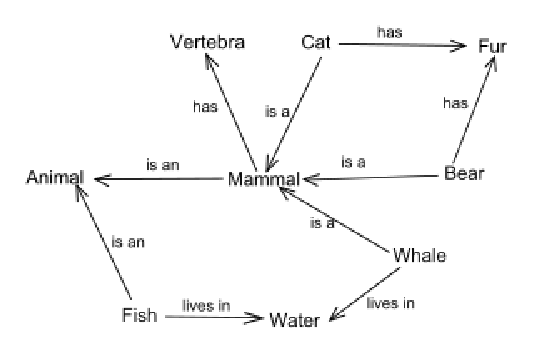
\includegraphics[height=0.75\textheight]{pics/Semantic_Net.eps}

\begin{itemize}
\item You need a very big graph to capture all meanings
\end{itemize}


\myslide{Wordnet in this course}


\begin{itemize}
\item We will use wordnet to test our skills in determining word meaning
  \begin{itemize}
  \item tag a short text from this year's story or stories
  \item discuss differences with other annotators
 \end{itemize}
\item As well as a source of examples and inspiration
\end{itemize}




\myslide{Synonyms for a \lex{dead} Parrot}

\begin{quote} \large
  \lex{be dead, be demised, be deceased, pass on, be no more, cease to be,
  expire, go to meet one's maker, be a stiff, be bereft of life,
  rest in peace, push up the daisies, one's metabolic processes are
  now history, be off the twig, kicked the bucket, shuffle off this
  mortal coil, ring down the curtain, join the choir invisible, be an
  ex-parrot}
\end{quote}

From the ``Dead Parrot Sketch'', also known as the ``Pet Shop Sketch''
or ``Parrot Sketch'', originally in \textit{Monty Python's Flying Circus},
first performed in the eighth episode of the show's first series,
"Full Frontal Nudity" (7 December 1969).

\section{Derivational Relations}

\myslide{Diathesis Alternations}

\MyLogo{\citet{Levin:1993}}

\begin{itemize}
\item \txx{Causative/inchoative alternation}:
  \begin{quote}
    \eng{Kim \ul{broke} the window} $\leftrightarrow$ \eng{The window \ul{broke}}
    \\ also \eng{the window \ul{is broken}} (state)
  \end{quote}
\item \txx{Middle construction alternation}:
  \begin{quote}
    \eng{Kim \ul{cut} the bread} $\leftrightarrow$ \eng{The bread \ul{cut} easily}
  \end{quote}
\item \txx{Conative alternation}:
  \begin{quote}
    \eng{Kim \ul{hit} the door} $\leftrightarrow$ \eng{Kim \ul{hit} at the door}
  \end{quote}
\item \txx{Body-part possessor ascension alternation}:
  \begin{quote}
    \eng{Kim \ul{cut} Sandy's arm} $\leftrightarrow$ \eng{Kim \ul{cut} Sandy on the arm}
  \end{quote}
\end{itemize}




\myslide{Diathesis Alternations and Verb Classes}

\MyLogo{\citet{Levin:1993}}

\begin{itemize}
\item A verb's (in)compatibility with different alternations is a strong
  predictor of its lexical semantics:
  \begin{quote}\smaller[1]
    \begin{tabular}{ccccc}
      & \lex{break} & \lex{cut} & \lex{hit} & \lex{touch} \\
      Causative & YES & NO & NO & NO \\
      Middle & YES & YES & NO & NO \\
      Conative & NO & YES & YES & NO \\
      Body-part & NO & YES & YES & YES \\
    \end{tabular}
    \vspace{3ex}

    \larger[1]
    \lex{break} = \{\eng{break, chip, crack, crash, crush, ...}\}\\
    \lex{cut} = \{\eng{chip, clip, cut, hack, hew, saw, ...}\}\\
    \lex{hit} = \{\eng{bang, bash, batter, beat, bump, ...}\}\\
    \lex{touch} = \{\eng{caress, graze, kiss, lick, nudge, ...}\}
  \end{quote}

\newpage


\item \textbf{Corollary}: we can predict the syntax of novel words we
  are given the semantic class for

\item The principal weakness of syntax-based verb classification is that
  there are often subtle divergences in semantics between synonyms (cf.\
  \lex{eat} vs.\ \lex{devour} vs.\ \lex{gobble})
\end{itemize}

\myslide{Agentive Nouns}
\MyLogo{}
\begin{itemize}
\item An \txx{agentive noun} is a word that is typically derived from
  another word denoting an action, and that identifies an entity that
  does that action.  \\ \textbf{verb} + \lex{-er, -or, -ant}
  \begin{exe}
    \ex \lex{murderer, commentator, whaler, director, computer}
    \ex ?? \lex{undertaker, cooker, footballer} (Saeed also includes these)
  \end{exe}
\item Should \lex{murderer} be listed separately from \lex{murder} in
the dictionary? Why or why not?
\item Also the undergoer: \textbf{verb} + \lex{-ee}: \lex{employee}
\end{itemize}

\myslide{Agentive Nouns in Other Languages}
\MyLogo{Thanks to Yeo Jia Qi (Malay)}

\begin{itemize}
\item Japanese (suffix distinguishes person/machine)
  \begin{itemize}
  \item \zh{運転する} → \zh{運転者} \jpn[driver]{unten-sha}
  \item \zh{計算する} → \zh{計算者} \zh{計算機} \jpn[computer]{keisan-sha/ki}
  \item \zh{研究する} → \zh{研究者} \zh{研究員} \jpn[researcher]{kenkyuu-sha/in}
  \item \zh{読む} → \zh{読み手} \zh{読者} \jpn[reader]{yomite/dokusha}
  \end{itemize}
\item Malay (prefix can convert any part  of speech)
  \begin{itemize}
  \item \zsm[help]{bantu (v)} → \zsm[assistant/helper]{pembantu} 
  \item \zsm[cut]{potong (v)} → \zsm[cutter (human/machine)]{pemotong}
  \item \zsm[fly]{terbang (v)} → \zsm[pilot (not passenger)]{penerbang}
  \item \zsm[scissors]{gunting (n)} → \zsm[(editor – human)]{penyunting}
  \end{itemize}

\end{itemize}
\myslide{Agentive Nouns in Other Languages}
\MyLogo{Thanks to Shalini (Tamil)}


\begin{itemize}\addtolength{\itemsep}{-1em}
\item Tamil, can convert verb or noun
  \begin{itemize}
  \item  \tam{வேலை} \eng[work]{vēlai} → \tam{வேலைக்காரர்} \eng[worker]{vēlaikkārar}
\item  \tam{சமையல்} \eng[cook]{samaiyal} → \tam{சமையல்காரர்} \eng[chef]{samaiyalkārar}
\item \tam{பாடல்} \eng[song]{pāl} → \tam{பாடகர்} \eng[singer]{pālkārar}
  \end{itemize}
\item Endings can mark gender, similar to pronouns
  \begin{itemize}
  \item Singer
    \begin{itemize}
    \item \tam{பாடகன்}   \eng{pāṭagan} (male)
    \item  \tam{பாடகி} \eng{pāṭaki} (female \ensuremath{\approx} male
      + \tam{இ} \eng{i} )
      \item  \tam{பாடகர்} \eng{pāṭaka} (formal)
    \end{itemize}
  \item Pronouns
    \begin{itemize}
    \item   \tam{அவன்} \eng[he]{avaṉ}
    \item   \tam{அவள்} \eng[she]{avaḷ}
    \item   \tam{அவர்} eng[they]{Avar} (Formal/Gender-neutral)
 
    \end{itemize}
  \end{itemize}
\end{itemize}

\section{Lexical Universals}

\myslide{Color Terms}

\begin{itemize}
\MyLogo{See also: \url{http://wals.info/chapter/133}: Colour Terms
by Paul Kay and Luisa Maffi}
\item \txx{Basic Color Terms}
  \begin{itemize}
  \item Monolexemic
  \item Not a hyponym of any other color
  \item Can be widely applied
  \item Not derived from a noun
  \end{itemize}
\item \txx{Focal Colors} are related to the neurophysiology of our visual system
\item Seem to come in an order \\
\hspace*{-4em}\makebox{$ \left\{ \begin{array}[c]{l}
    \mbox{\con{white/dark}} \\  \mbox{\con{black/light}}
  \end{array} \right\}
   < \mbox{\con{red}} < 
 \left\{ \begin{array}[c]{l}
    \mbox{\con{green}} \\  \mbox{\con{yellow}}
  \end{array} \right\}
 < \mbox{\con{blue}} < \mbox{\con{brown}} <  
\left\{ \begin{array}[c]{l}
    \mbox{\con{purple}} \\  \mbox{\con{pink}} \\ \mbox{\con{orange}} \\  \mbox{\con{grey}}
  \end{array} \right\} $}
\end{itemize}

\myslide{Core Vocabulary}
\MyLogo{\url{en.wiktionary.org/wiki/Appendix:Swadesh_list}}
\begin{itemize}
\item Some universal terms can be used to compare languages
  \begin{itemize}
  \item lexicostatistics (quantitative language relatedness assessment)
  \item glottochronology (language divergence dating)
\end{itemize}
\item The \txx{Swadesh list}, developed by Morris Swadesh from 1940 onward 
\end{itemize}
\vspace*{-2ex}
I, You, we, this, that, who, what, not, all, many, one, two, big,
long, small, woman, man, person, fish, bird, dog, louse, tree, seed,
leaf, root, bark, skin, flesh, blood, bone, grease, egg, horn, tail,
feather, hair, head, ear, eye, nose, mouth, tooth, tongue, claw, foot,
knee, hand, belly, neck, breasts, heart, liver, drink, eat, bite, see,
hear, know, sleep, die, kill, swim, fly, walk, come, lie, sit, stand,
give, say, sun, moon, star, water, rain, stone, sand, earth, cloud,
smoke, fire, ash(es), burn, path, mountain, red, green, yellow, white,
black, night, hot, cold, full, new, good, round, dry, name
\vspace*{-1ex}
\begin{itemize}
\item Available in many languages (hundreds); Now linked to wordnet 
\end{itemize}
\vspace*{-1ex}


\myslide{Natural Semantic Meta Language}
\MyLogo{\citet{AnnaW:1996}}
\begin{itemize}
\item Try to define everything in terms of semantic primitives and reductive paraphrase
  \begin{itemize}
  \item simple, indefinable, and universally lexicalized concepts
  \item breaking complex concepts down into simpler concepts
  \end{itemize}
\end{itemize}
\begin{verbatim}
X feels unhappy=
sometimes a person thinks something like this:
    something bad happened to me
    I don’t want this	
    if I could, I would do something
because of this, this person feels something bad
X feels like this
\end{verbatim}
\begin{itemize}
\item Very hard to do consistently and reproducibly
\end{itemize}

\myslide{The Semantic Primitives}
\setlength{\columnsep}{1em}
\begin{multicols}{2} \small
\begin{itemize}
\item \textbf{substantives}: 
    I, YOU, SOMEONE, PEOPLE, SOMETHING/THING, BODY
\item \textbf{relational substantive}: 
    KIND, PART
\item \textbf{determiners}: 
    THIS, THE SAME, OTHER/ELSE
\item \textbf{quantifiers}: 
    ONE, TWO, MUCH/MANY, SOME, ALL
\item \textbf{evaluators}: 
    GOOD, BAD
\item \textbf{descriptors}: 
    BIG, SMALL
\item \textbf{mental predicates}: 
    THINK, KNOW, WANT, FEEL, SEE, HEAR
\item \textbf{speech}: 
    SAY, WORDS, TRUE
\item \textbf{actions, events, movement, contact}: 
    DO, HAPPEN, MOVE, TOUCH
\item \textbf{location, existence, possession, specification}: 
    BE (SOMEWHERE), THERE IS, HAVE, BE (SOMEONE/THING)
\item \textbf{life and death}: 
    LIVE, DIE
\item \textbf{time}: 
    WHEN/TIME, NOW, BEFORE, AFTER, A LONG TIME, A SHORT TIME, FOR SOME TIME, MOMENT
\item \textbf{space}: 
    WHERE/PLACE, HERE, ABOVE, BELOW, FAR, NEAR, SIDE, INSIDE
\item \textbf{logical concepts}: 
    NOT, MAYBE, CAN, BECAUSE, IF
\item \textbf{intensifier, augmentor}: 
    VERY, MORE
\item \textbf{similarity}: 
    LIKE/WAY 
  \end{itemize}
  \end{multicols}
% \section{Problems}
% \MyLogo{}

% \myslide{Synonymy/Antonymy}
%   \begin{enumerate}
%   \item Find a pair of absolute synonyms in a language that you speak.
%   \item Decide if the words in the following sets are absolute synonyms,
% near synonyms or partial synonyms. How do you decide? What
% type of criteria have you used?
% \begin{exe}
%   \ex \lex{tell, say, talk}
%   \ex \lex{sad, unhappy}
% \end{exe}
% \newpage
% \item Classify the following pairs of opposites
% \begin{exe}
%   \ex \lex{temporary/permanent}
%   \ex \lex{strong/weak}
%   \ex \lex{open/shut}
%   \ex \lex{monarch/subject} 
%   \ex \lex{advance/retreat}
%   \ex \lex{buyer/seller}
%   \ex \lex{clean/dirty}
%   \ex \lex{present/absent} 
%   \ex \lex{red/green}
%   \ex \lex{yesterday/today}
% \end{exe}
% \end{enumerate}

% \myslide{Agentive Nouns}
% Below are some nouns ending in \lex{-er} and \lex{-or}. Using your intuition
% about their meanings, discuss their status as agentive nouns. In
% particular, are they derivable by regular rule or would they need to
% be listed in the lexicon?
% \begin{quote}
% \lex{author, blazer, blinker, choker, crofter, debtor, loner, mentor,
% reactor, roller, lecturer}
% \end{quote}
% Check your decisions against a dictionary's entries.

% \myslide{Other Relations}
% For the following sets of sentences, discuss the meaning relations
%   between the underlined words.
%   \begin{exe}
%     \ex 
%     \begin{xlist}
%       \ex \eng{The wind \ul{shut} the door.}
%       \ex \eng{The door \ul{shut} with a bang.}
%     \end{xlist}
%     \ex 
%     \begin{xlist}
%       \ex \eng{The student \ul{slept} all through the class.}
%       \ex \eng{The student \ul{snored} all through the class.}
%     \end{xlist}
%    \ex 
%     \begin{xlist}
%       \ex \eng{Kim \ul{bought} a text book from Sandy.}
%       \ex \eng{Sandy \ul{sold} a textbook to Kim.}
%       \ex \eng{Kim \ul{obtained} a text book from Sandy.}
%     \end{xlist}
%    \ex 
%     \begin{xlist}
%       \ex \eng{Bobby \ul{showed} her answers to  Hiromi.}
%       \ex \eng{Hiromi \ul{saw} Bobby's answers.}
%       \ex \eng{Hiromi \ul{looked at} Bobby's answers.}
%     \end{xlist}
%   \end{exe}



\myslide{Acknowledgments and References}

\begin{itemize}
\item Definitions from WordNet: \url{http://wordnet.princeton.edu/}
\item Images from
  \begin{itemize}
  \item the Open Clip Art Library: \url{http://openclipart.org/}
  \item Steven Bird, Ewan Klein, and Edward Loper (2009) 
     \textit{Natural Language Processing with Python}, O'Reilly Media
    \\ \url{www.nltk.org/book}
\end{itemize}
%\item Problems  partially based on exercises from Saeed (2003)
\item Video: Dead parrot sketch Monty Python
\end{itemize}

%\myslide{Bibliography}
% Reading: Jurafsky and Martin (2008) Chapter 20
\small
\bibliographystyle{aclnat}
\bibliography{abb,mtg,nlp,ling}

\clearpage
%\end{CJK}
\end{document}


%%% Local Variables: 
%%% coding: utf-8
%%% mode: latex
%%% TeX-PDF-mode: t
%%% TeX-engine: xetex
%%% End: 

